\section{Results}

We ran our analysis over most of the SPEC CPU 2000 integer benchmarks, using the MinneSPEC reduced data input set \cite{KleinOsowski02minnespec}.
The results for our baseline model, along with the descriptions of the benchmarks as provided by SPEC \cite{henning00spec}, are provided in Table \ref{baseline}.
From these results we observe that there is not a great deal of task-level parallelism in these programs, at least in our baseline model.
We will now proceed to describe the effects of different dependency models on our limits of parallelism, noting that while parallelism does not exceed single figures for any of the models we examine here, gains in relative terms will still give us insight on promising directions in thread extraction.

\begin{table*}
\begin{tabular}{ | l | l | l | r | r | r | }
\hline
Benchmark & Language & Description & Serial length & Critical path length & Parallelism \\
\hline
164.gzip & C & Compression & 852994275 & 836250530 & 1.020 \\
175.vpr\_place & C & FPGA Circuit Placement & 30015847 & 28888197 & 1.039 \\
175.vpr\_route & C & FPGA Circuit Routing & 9008077 & 6688489 & 1.347 \\
176.gcc & C & C Programming Language Compiler & 102875883 & 83960956 & 1.225 \\
181.mcf & C & Combinatorial Optimization & 160615720 & 74266623 & 2.163 \\
186.crafty & C & Game Playing: Chess & 166315214 & 153019717 & 1.087 \\
197.parser & C & Word Processing & 391853645 & 361559175 & 1.084 \\
252.eon\_cook & C++ & Computer Visualization & 396417460 & 178717581 & 2.218 \\
252.eon\_kajiya & C++ & Computer Visualization & 528195627 & 251127042 & 2.103 \\
252.eon\_rushmeier & C++ & Computer Visualization & 383335201 & 168056567 & 2.281 \\
253.perlbmk & C & PERL Programming Language & 194675347 & 192775902 & 1.010 \\
254.gap & C & Group Theory, Interpreter & 80099675 & 75660828 & 1.059 \\
255.vortex & C & Object-oriented Database & 97266720 & 80887698 & 1.202 \\
300.twolf & C & Place and Route Simulator & 129292883 & 117049408 & 1.105 \\
\hline
\end{tabular}
\caption{Description of and baseline figures for the SPEC CPU 2000 integer benchmarks}
\label{baseline}
\end{table*}

\subsection{Data dependencies}

\begin{figure}
 \centering
 \includegraphics[width=3in]{spec-data}
 \caption{Limits of parallelism with static and dynamic data dependencies}
 \label{spec-data}
\end{figure}

Figure \ref{spec-data} shows the parallelism limits when considering static and dynamic data dependencies.
It is perhaps surprising to note that for many benchmarks the use of dynamic dependencies does not give much of an advantage over static dependencies (in fact only a 3.3\% speed-up on average over baseline), suggesting that dependencies are perhaps fairly consistent over the execution of a program.

\subsection{Control dependencies}

\begin{figure}
 \centering
 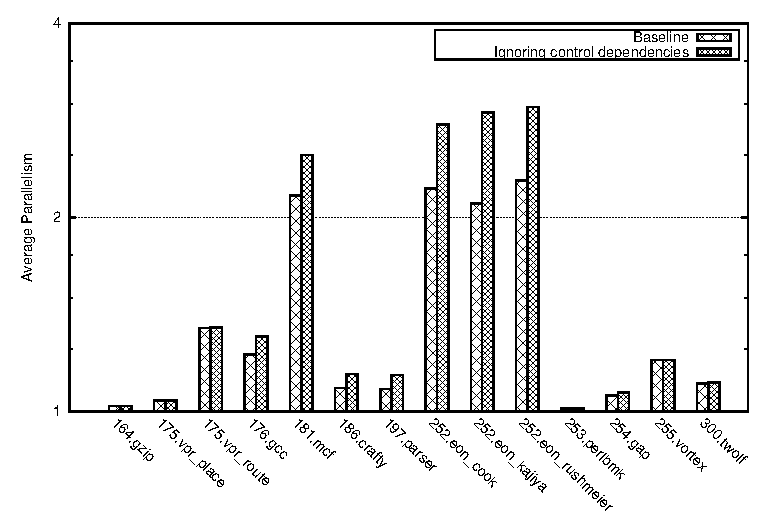
\includegraphics[width=3in]{spec-ctl}
 \caption{Limits of parallelism with and without static control dependencies}
 \label{spec-ctl}
\end{figure}

Figure \ref{spec-ctl} compares the limits of parallelism under the two control dependency models.
Ignoring control dependencies models the effects of perfect control speculation.
Here we see that a few benchmarks show a significant improvement, at least in relative terms, when control dependencies are ignored---an average speed-up of 9.2\% over the baseline.
These suggest that control speculation is a valuable technique for increasing parallel performance.
As noted, simple branch prediction (e.g.\ predicting the same branch as the one last taken) is sufficient for high accuracy \cite{smith98study}, and consequently we believe that such improvements should be attainable.

\subsection{Line-level parallelism}

\begin{figure}
 \centering
 \includegraphics[width=3in]{spec-gran}
 \caption{Limits of parallelism of different granularities}
 \label{spec-gran}
\end{figure}

We now move on to looking at limits of parallelism for different levels of granularity, beginning with line-level parallelism, which is the amount of parallelism achievable if every line can be spawned.
So far we have restricted ourselves to spawning function calls only, so the line-level model subsumes the task-level one.
The parallelism found includes function-call-level parallelism, as well as task-level parallelism where task boundaries do not have to be function calls.
Unfortunately, however, it also includes inter-line instruction-level parallelism, which may be too fine-grain for any multi-core processors to exploit---the spawning of single lines like \texttt{x++;} would probably worsen performance.
This model also does not in general include loop-level parallelism, as we cannot distinguish between loop-independent and loop-carried dependencies.

Figure \ref{spec-gran} shows the improvement in parallelism, which averages 91\%.
Some benchmarks which thus far have displayed hardly any parallelism begins to exhibit more, although it is still low in absolute terms.
It suggests that perhaps we should look closer at other ways of delineating tasks in addition to using function calls.

\subsection{Loops}

Figure \ref{spec-gran} also shows the limits of parallelism when natural loop iterations are also considered as tasks.
It shows the effects of exploiting DOALL parallelism, where loop iterations that are completely independent from each other can be executed in parallel.
At the same time, however, spawning a task for each loop iteration means that if there are cross-iteration dependencies then no parallelism is possible, thus precluding DOACROSS parallelism or software pipelining.
The balance between DOALL and DOACROSS loops would then determine whether parallelism rises or falls compared to the baseline.

The results, as expected, show a mixed picture.
Benchmarks such as gzip and twolf show a marked improvement, as they appear to have a few DOALL loops.
Others, such as mcf and eon, show an even bigger degradation, due to the presence of DOACROSS parallelism.
It would be interesting to explore the limits of parallelism when only iterations of loops with no loop-carried dependencies are spawned, allowing us to have the best of both worlds.

\subsection{Spawn hoisting}

\begin{figure}
 \centering
 \includegraphics[width=3in]{spec-hoist}
 \caption{Limits of parallelism with and without hoisting spawns}
 \label{spec-hoist}
\end{figure}

The effects of spawn hoisting are presented in Figure \ref{spec-hoist}, which shows the limits of parallelism with and without the optimisation.
While spawn hoisting is useful in the eon benchmark in particular, for most cases the difference it makes is marginal.
On average it results in a 5.5\% speed-up over the baseline.
Nevertheless, this appears to be a relatively straightforward optimisation with few overheads incurred, and as such there is no reason for it to be excluded when performing thread extraction.

\subsection{Other benchmarks}

\subsection{Validation}

\begin{figure}
 \centering
 \includegraphics[width=3in]{cilk}
 \caption{Limits of parallelism in Cilk programs}
 \label{cilk}
\end{figure}

To ensure that our model can discover all of the parallelism expressible using popular thread libraries we used a number of example Cilk programs packaged with the version 5.4.6 release of Cilk, the results of which are displayed in Figure \ref{cilk}.
The leftmost column shows the span measurement that Cilk performs when running these programs on a four-core Linux machine, showing the maximum speed-up given a sufficient number of processors.
The others show the results of running Embla over the same programs with the Cilk keywords removed, i.e.\ their sequential versions.
The span measured by Cilk is in general comparable to the limits computed by Embla using the baseline model, which is the most similar model---this validates that Embla is able to find most if not all of the parallelism expressible in Cilk.
In fact, our results show there is still room for improvement if we allow loop-level parallelism, which Cilk currently does not support\footnote{We note however that Cilk++, a commercialised version, does support parallel for-loops.}.

It can be easily seen by looking at the scale of the y-axis that potential parallelism for most of these programs is much higher than that in the SPEC suite.
This suggests that while a small number of programs have lots of inherent task-level parallelism, general-purpose programs that are not `embarrassingly parallel' have little and cannot be easily transformed into highly concurrent programs, at least not by simple additions of thread library keywords.

\subsection{Discussion}

We now describe why some of these programs exhibit such low levels of parallelism, and suggest what can be done to increase their potential.
